\documentclass[12pt]{article}
\usepackage{amssymb, amsmath,amsfonts}
\usepackage{tikz}
\usepackage{pgfplots}
\usepackage[pdftex, bookmarks=true,colorlinks,linkcolor=red,urlcolor=blue,citecolor=blue]{hyperref}
\usepackage{tikz}

\begin{document}

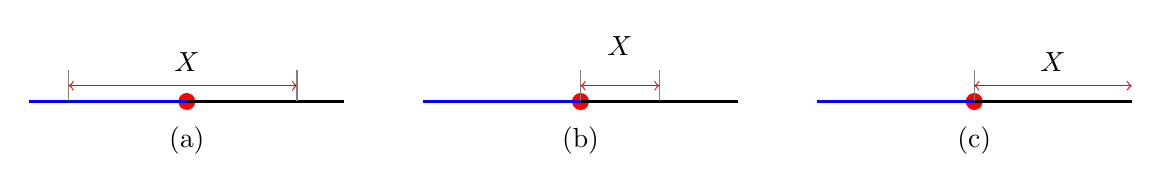
\begin{tikzpicture}
\draw [fill,color=red] (2,0) circle [radius=0.1];
\draw[very thick,color=blue] plot coordinates {(0,0)(2,0)};
\draw[very thick,color=black] plot coordinates {(2,0)(4,0)};
\draw[color=gray] plot coordinates {(0.5,0)(0.5,0.4)};
\draw[color=gray] plot coordinates {(3.4,0)(3.4,0.4)};
\draw[color=red] [<->] (0.5,0.2) -- (3.4,0.2);
\node[color=black] at (2.0,0.5) {$X$};
\node[color=black] at (2.0,-0.5) {(a)};

\draw [fill,color=red] (7,0) circle [radius=0.1];
\draw[very thick,color=blue] plot coordinates {(5,0)(7,0)};
\draw[very thick,color=black] plot coordinates {(7,0)(9,0)};
\draw[color=gray] plot coordinates {(7,0)(7,0.4)};
\draw[color=gray] plot coordinates {(8,0)(8,0.4)};
\draw[color=red] [<->] (7,0.2) -- (8,0.2);
\node[color=black] at (7.5,0.7) {$X$};
\node[color=black] at (7.0,-0.5) {(b)};

\draw [fill,color=red] (12,0) circle [radius=0.1];
\draw[very thick,color=blue] plot coordinates {(10,0)(12,0)};
\draw[very thick,color=black] plot coordinates {(12,0)(14,0)};
\draw[color=gray] plot coordinates {(12,0)(12,0.4)};
\draw[color=gray] plot coordinates {(3.4,0)(3.4,0.4)};
\draw[color=red] [<->] (12,0.2) -- (14,0.2);
\node[color=black] at (13,0.5) {$X$};
\node[color=black] at (12,-0.5) {(c)};

\end{tikzpicture}

\end{document}